\documentclass[10pt]{article}
\usepackage{amsmath,textcomp,amssymb,geometry,graphicx,enumerate,tikz,algorithm,algpseudocode,pifont}
\usetikzlibrary{calc}
\usetikzlibrary{datavisualization}
\usetikzlibrary{datavisualization.formats.functions}


\textheight=9in
\textwidth=7in
\topmargin=-.75in
\oddsidemargin=-0.25in
\evensidemargin=-0.25in

\usepackage{listings}
\lstnewenvironment{codeblock}
    {\lstset{language=Python,
      showspaces=false,
      showtabs=false,
      breaklines=true,
      mathescape=true,
      showstringspaces=false,
      breakatwhitespace=true,
      commentstyle=\textit,
      keywordstyle=\textbf,
      basicstyle=\ttfamily,
      escapechar=`,
      moredelim={**[is][{\color{RoyalBlue}}]{\^^M\\beginsol}{\^^M\\endsol}},
      moredelim={[is][{\color{RoyalBlue}}]{\^^M\\beginexp}{\^^M\\endexp}},
    }}
    {}

\begin{document}
\section*{03/07/2016}
	\subsection*{Ridge Regression} (aka Tikhonov regularization)
	\
	\begin{itemize}
		\item (1) + (A) + $\ell_{2}$ penalized mean loss (d).
		\item Optimization problem $J(w)$:
		\begin{center}
			\begin{tabular}{|c|}
				\hline
				Find $w$ that minimizes
				$|Xw - y|^{2} + \lambda||w'||^{2}$\\
				\hline
			\end{tabular}\\
		\end{center}
		Where $w'$ is $w$ with components $\alpha$ replaced by 0. $X$ has fictitious dimension but we DON'T penalize $\alpha$.
		\item Adds a penalty term to encourage small $|w'|$ -- called \underline{shrinkage}.
		\item Why? Guaranteed positive definite normal equations; always unique solution. e.g. when $d>n$ always semi-definite.
			\begin{center}
				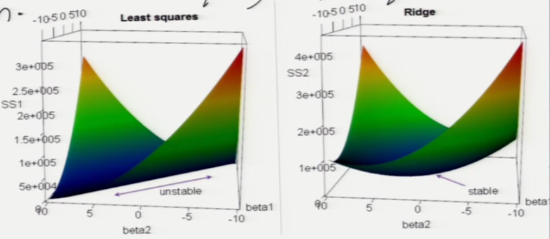
\includegraphics[scale=0.5]{../images/ridge}
			\end{center}
		\item Reduces over-fitting by reducing variance by penalizing large weights.
			\begin{center}
				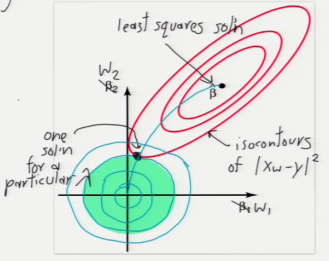
\includegraphics[scale=0.5]{../images/sqrsvslambda}
			\end{center}
		\item Setting $\nabla J = 0$ gives equations,
			\begin{align*}
				(X^{T}X + \lambda I')w = X^{T}y
			\end{align*} 
		\item where $I'$ is identity matrix with bottom right set to zero.
		\item Algorithm: solve for $w$. Return $h(z) = w^{T}x$.
		\item Increasing $\lambda \Rightarrow$ more \underline{regularization}; smaller $|w'|$.
		\item Given our data model $y = Xv + e$, where $e$ is noise.
		\item Variance of ridge regression is Var($x^{T}(X^{T}X + \lambda I')^{-1}X^{T}e)$.
		\item As $\lambda \rightarrow \infty$, variance $\rightarrow 0$, but bias increases.
			\begin{center}
				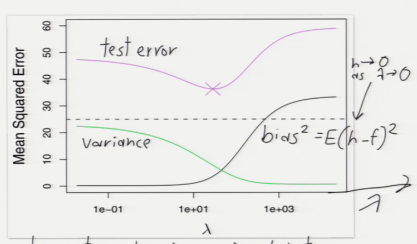
\includegraphics[scale=0.5]{../images/lambdabiasvsvariance}
			\end{center}
		\item $\lambda$ is a hyper-parameter; tune by (cross)-validation.
		\item Ideally features should be "normalized" to have same variance.
		\item Alternative: Use asymmetric penalty by replacing $I'$ with other diagonal matrix.
	\end{itemize} 
	
	\subsection*{Bayesian justification for ridge regression}
	\
	\begin{itemize}
		\item Assign a prior probability on $w'$: a Gaussian centered at 0.
		\item Posterior probability $\approx$ likelihood of $w \cdot $ prior $P(w') \leftarrow$ Gaussian PDF. 
		\item Maximize the log posterior, $\ell$n likelihood + $\ell n P(w') =$ -const$|Xw-y|^{2}$ - const$|w'|^{2}$ - constant.
		\item This method (using likelihood, but maximizing posterior) is called \underline{maximum a posteriori} (MAP).
	\end{itemize}
	
	\subsection*{Kernels}
	\
	\begin{itemize}
		\item Recall: with $d$ input features, degree-p polynomials blow up to $\mathcal{O}(d^{p})$ features.
		\item Today we use magic to use those features without computing them!
		\item Observation: In many learning algorithms:
			\begin{itemize}
				\item The weights can be written as a linear combination of input samples.
				\item We can use inner products of $\phi(x)'$s only $\Rightarrow$ don't need to compute $\phi(x)$!
				\item Suppose $w = X^{T}a = \sum_{i=1}^{n} a_{i}X_{i}$ for some $a \in \mathbb{R}^{n}$.
				\item Substitute this identity into algorithms and optimize $n$ \underline{dual weights} (aka \underline{dual parameters} a, instead of $d+1$ \underline{primal weights} w.
			\end{itemize}
	\end{itemize}
	
	\subsection*{Kernel Ridge Regression}
	\
	\begin{itemize}
		\item \underline{Center} $X$ and $y$ so their means are zero; $X_{i} \leftarrow X_{i} - \mu_{x}$. By centering the matrix we minimize the penalization of $\alpha$
		\item This lets us replace $I'$ with $I$ in normal equations:
			\begin{align*}
				&(X^{T}X + \lambda I)w = X^{T}y\\
				&\Rightarrow w = \frac{1}{\lambda}(X^{T}y - X^{T}Xw) = X^{T}a  \ \ \ \ \ \text{where } a = \frac{1}{\lambda}(y-Xw)
			\end{align*}
		\item This shows that $w$ is a linear combination of samples. To compute $a$:
			\begin{align*}
				\lambda a = (y - XX^{T}a) \Rightarrow a = (XX^{T} + \lambda I)^{-1}y
			\end{align*}
		\item $a$ is the \underline{dual solution}; solves the \underline{dual form} of ridge regression:
		\begin{center}
			\begin{tabular}{|c|}
				\hline
				Find $a$ that minimizes $|XX^{T} - y|^{2} + \lambda|X^{T}a|^{2}$\\
				\hline
			\end{tabular}\\
		\end{center}
		\item Regression function is:
			\begin{align*}
				h(z) = w^{T}z = a^{T}Xz = \sum_{i=1}^{n} a_{i}(X_{i}^{T}z) \Leftarrow \text{weighted sum of inner products}
			\end{align*}
		\item Let $k(x, z) = x^{T}z$ be \underline{kernel function}.
		\item Let $K = XX^{T}$ be nxn \underline{kernel matrix}. Note $K_{ij} = k(X_{i}, X_{j})$.
		\item $K$ is singular if $n>d$. In that case no solution if $\lambda = 0$.
		\item Summary of kernel ridge regression:
			\begin{itemize}
				\item Solve $(K + \lambda I)a = y$  for a $\Leftarrow \mathcal{O}(n^{3})$ time.
				\item $K_{ij} = k(X_{i}, X_{j}) \ \forall i,j \Leftarrow \mathcal{O}(n^{2}d)$ time.
				\item for each test point $z$: $h(z) = \sum_{i=1}^{n} a_{i} k(X_{i}, z) \Leftarrow \mathcal{O}(nd)$ time.
			\end{itemize}
		\item Do not use $X$ directly: only $k(\cdot , \cdot)$.
		\item Dual: solve $n$x$n$ linear system.
		\item Primal: solve $d$x$d$ linear system.
	\end{itemize}
	
	\subsection*{The Kernel Trick} (aka \underline{kernelization})
	\
	\begin{itemize}
		\item The \underline{polynomial kernel} of degree $p$ is $k(x,z) = (x^{T}z + 1)^{p}$.
		\item Theorem: $(x^{T}z + 1)^{p} = \phi(x)^{T}\phi(z)$ where $\phi(x)$ contains every monomial in $x$ of degree $0 \dots p$.
		\item Example for $d=2, p=2$.
			\begin{align*}
				(x^{T}z+1)^{2} &= x_{1}^{2}z_{1}^{2} + x_{2}^{2}z_{2}^{2} + 2x_{1}z_{1}x_{2}z_{2} + 2x_{1}z_{1} + 2x_{2}z_{2} + 1\\
					& = \begin{bmatrix}
						x_{1}^{2} & x_{2}^{2} & \sqrt{2x_{1}x_{2}} & \sqrt{2x_{1}} & \sqrt{2x_{2}} & 1
					\end{bmatrix}
					\cdot
					\begin{bmatrix}
						z_{1}^{2}\\
						z_{2}^{2}\\
						\sqrt{2z_{1}z_{2}}\\
						\sqrt{2z_{1}}\\
						\sqrt{2z_{2}}\\
						1\\
					\end{bmatrix}\\
					&= \phi(x)^{T} \phi(z)\\
			\end{align*}
		\item Key win: compute $\phi(x)^{T} \phi(z)$ in $\mathcal{O}(d)$ time instead of $\mathcal{O}(d^{p})$ even though $\phi(x)$ has length $\mathcal{O}(d^{p})$.
		\item Kernel ridge regression replaces $X_{i}$ with $\phi(X_{i})$:
			\begin{itemize}
				\item Let $k(x, z) = \phi(x)^{T}\phi(z)$.	
			\end{itemize} 
	\end{itemize}
\end{document}